\documentclass[../../Thesis.tex]{subfiles}
\usepackage[italian]{babel}

\begin{document}
\chapter{Metodologia}
Questa sezione descrive in dettaglio l'approccio seguito per affrontare il problema della classificazione degli smart contracts. Questo capitolo è fondamentale per comprendere come sono stati raccolti, pre-processati e utilizzati i dati, come è sono stati configurati e addestrati i modelli e quali strumenti e tecniche sono stati impiegati per ottenere i risultati presentati.

La metodologia adottata in questa tesi è suddivisa nelle seguenti fasi principali:
\begin{enumerate}
    \item Raccolta e preparazione dei dati: esplorazione del dataset utilizzato, delle tecniche di pre-processing applicate e delle modalità di suddivisione dei dati per l'addestramento e la valutazione.
    \item Modellazione: descrizione dell'architettura dei modelli utilizzati, delle scelte di configurazione e delle strategie di addestramento.
.
\end{enumerate}
Ogni fase sarà trattata in modo dettagliato, evidenziando le scelte metodologiche compiute e le motivazioni alla base di tali scelte. Questo approccio sistematico garantisce trasparenza e replicabilità del lavoro svolto, consentendo ad altri  di comprendere e, eventualmente, replicare i risultati ottenuti.
    
\section{Esplorazione dei dati}
Il dataset \cite{rossini2022slitherauditedcontracts} utilizzato in questo progetto è un dataset disponibile pubblicamente sulla piattaforma HuggingFace una delle più importanti piattaforme per il Natural Language Processing. HF è un'infrastruttura open-source che fornisce accesso a una vasta gamma di modelli di deep learning pre-addestrati, tra cui alcuni dei più avanzati nel campo del NLP.
Questo dataset contiene informazioni su 106.474 SmartContracts pubblicati sulla rete Ethereum. Ogni elemento nel dataset è composto da quattro elementi:
\begin{itemize}
    \item  \textbf{Address}: l'indirizzo del contratto
    \item  \textbf{SourceCode}: il codice sorgente del contratto, scritto in linguaggio Solidity
    \item  \textbf{ByteCode}: il codice bytecode del contratto, ottenuto a partire dalla compilazione del codice sorgente utilizzando il compilatore di Solidity. Questo bytecode è quello che viene eseguito sulla macchina virtuale di Ethereum (EVM).
    \item  \textbf{Slither}: il risultato dell'analisi statica del contratto con Slither, un tool open-source per l'analisi statica di contratti scritti in Solidity. Questo risultato è un array di valori che vanno da 1 a 5, dove ogni numero  rappresenta la presenza di una vulnerabilità e 4 rappresenta un contratto safe, cioè privo di vulnerabilità.
\end{itemize}
Le vulnerabilità che sono state prese in questo lavoro sono le seguenti:
\begin{itemize}
    \item Access-Control
    \item Arithmetic
    \item Other
    \item Reentrancy
    \item Safe
    \item Unchecked-Calls
\end{itemize}
Prima della costruzione dei modelli è stata affrontata una fase di analisi esplorativa dei dati. Questa fase è stata svolta per comprendere meglio la struttura del dataset e dei contratti da classificare, per individuare eventuali problemi. A livello pratico, questa fase di analisi esplorativa dei dati è stata eseguita utilizzando il linguaggio Python, con l'ausilio di librerie come Pandas, NumPy, Matplotlib e Seaborn per l'analisi e la visualizzazione dei dati.
Il dataset è diviso in tre sottoinsiemi: training, validation e test set.
Il dataset di training è composto da 79.641 contratti, il dataset di validazione da 10.861 contratti e il dataset di test da 15.972 contratti.
Tutte le informazioni sono presenti per tutti i contratti tranne l'informazione relativa al bytecode, che risulta assente per 227 contratti nel training set, 30 nel validation set e 51 nel test set. Durante la fase di preprocessing questi contratti sono stati rimossi dal dataset. 
 
Per ottenere una visione d'insieme delle lunghezze dei contratti, abbiamo calcolato la lunghezza media del source code e del bytecode. Prima del preprocessing le lunghezze medie di SourceCode e ByteCode sono rispettivamente di 3155 token e 8114 token.
Abbiamo visualizzato la distribuzione delle lunghezze del source code utilizzando un istogramma. Per migliorare la leggibilità del grafico, abbiamo raggruppato i dati per quanto riguarda il source code in intervalli di 500 token. L'istogramma è accompagnato da una linea che indica la lunghezza media dei token rappresentata con una linea tratteggiata rossa.

L'inclusione delle lunghezze medie fornisce un punto di riferimento utile per interpretare le distribuzioni e confrontare i singoli esempi di codice rispetto alla media del dataset. Queste analisi sono fondamentali per le successive fasi di preprocessing e modellazione, garantendo che i modelli possano gestire efficacemente la variabilità presente nei dati.
Sul bytecode non è stato applicato nessun tipo di preprocessing per ridurre la dimensione dei dati. Per quanto riguarda il codice sorgente sono stati eliminati tutti i commenti e le funzioni getter monoistruzione, cioè tutte quelle funzioni \texttt{getX()} le quali abbiano come unica istruzione una istruzione di return, poichè sono state assunte come funzioni corrette, l'eliminazione di queste stringhe è avvenuta tramite una ricerca delle stringhe effettuata con una regex.
Abbiamo unito i set di dati di addestramento, test e validazione in un unico DataFrame per analizzare le lunghezze del source code e del bytecode. In particolare, sono state calcolate rispettivamente le lunghezze del codice sorgente e del bytecode. Effettuando le rimozioni dei commenti la media del numero di token del sourcecode scende a 1511 token, mostrando come la rimozione dei commenti abbia un grande impatto sulla lunghezza media del codice. Rimuovendo anche le funzioni getter monoistruzione la lunghezza media del source code scende a 1481 token.
\begin{figure}[htbp]
    \centering
    \begin{subfigure}[b]{0.49\textwidth}
        \centering
        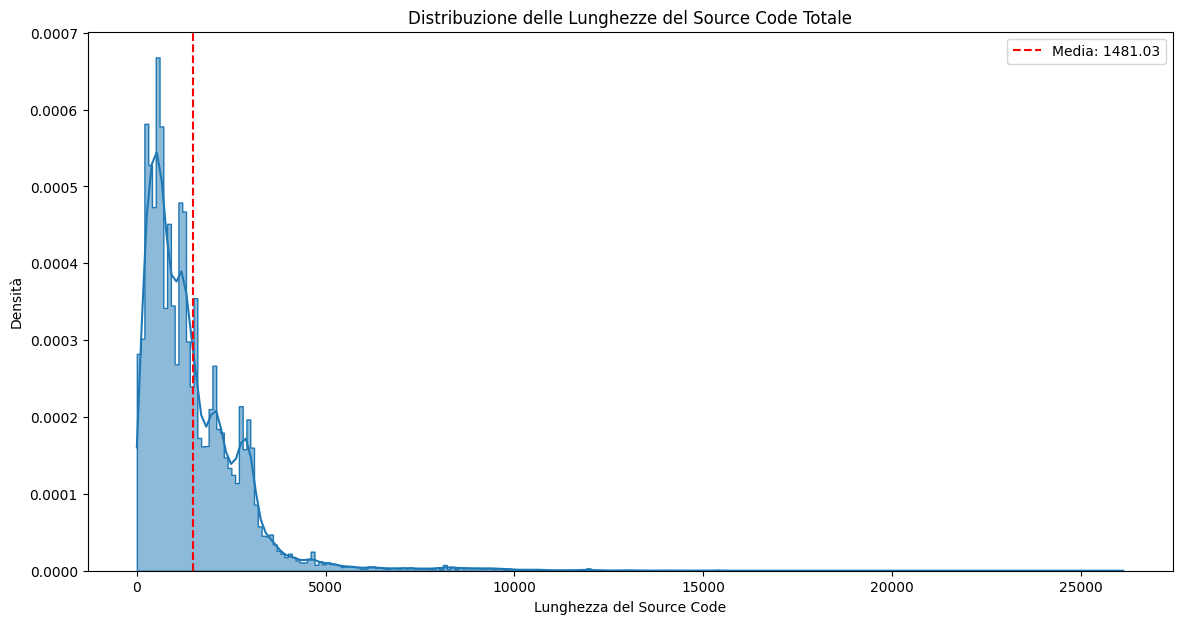
\includegraphics[width=\textwidth]{../../img/SCTokensPreprocessed.png}
        \caption{Distribuzione delle Lunghezze del Source Code dopo il preprocessing}
        \label{fig:sourcecode_length_distribution}
    \end{subfigure}
    \hfill
    \begin{subfigure}[b]{0.49\textwidth}
        \centering
        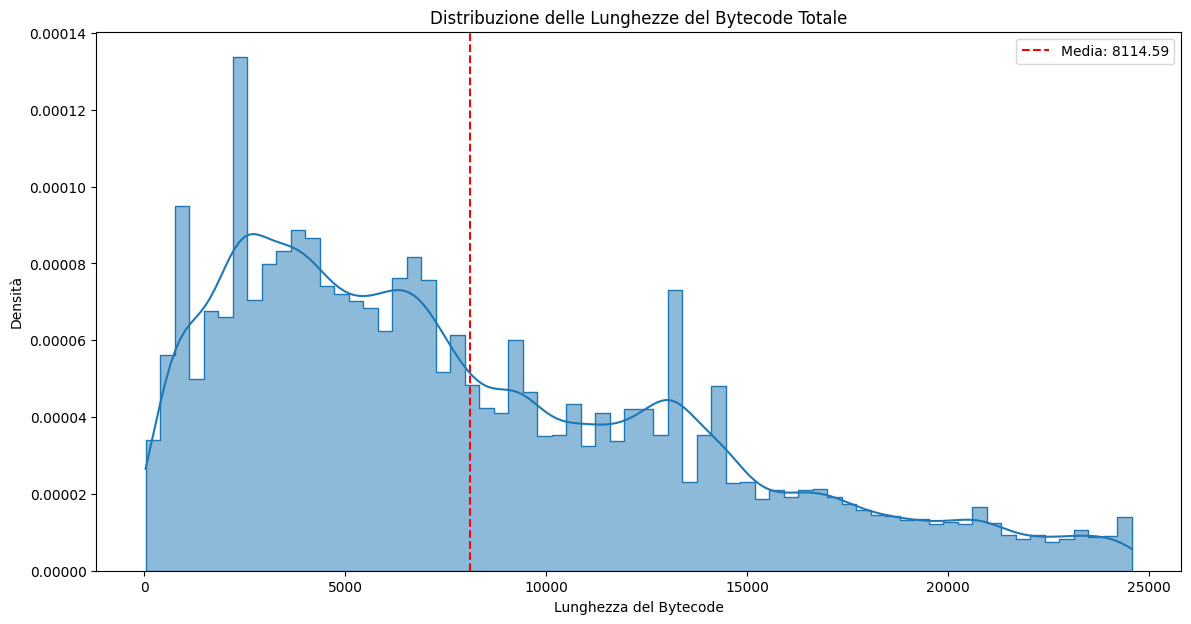
\includegraphics[width=\textwidth]{../../img/BCTokensPreprocessed.png}
        \caption{Distribuzione delle Lunghezze del Bytecode dopo il preprocessing}
        \label{fig:bytecode_length_distribution}
    \end{subfigure}
    \caption{Distribuzioni delle lunghezze del source code e del bytecode.}
    \label{fig:length_distributions}
\end{figure}
Successivamente, la fase di esplorazione dei dati ha previsto l'analisi delle classi di vulnerabilità dei dati. 

\subsection{Distribuzione delle Classi e Matrici di Co-occorrenza}

In questa sezione, presentiamo la distribuzione delle classi e le matrici di co-occorrenza per i dataset di addestramento, test e validazione. Si precisa che i risultati di seguito proposti si riferiscono già al dataset da cui sono stati sottratti i contratti privi di bytecode.

\subsubsection{Distribuzione delle Classi}

La Tabella \ref{tab:class_distribution} mostra la distribuzione delle classi per i tre dataset. È evidente che la classe 'unchecked-calls' è la più frequente in tutti e tre i dataset, mentre la classe 'access-control' è la meno rappresentata.
\begin{table}[h!]
    \centering
    \begin{tabular}{|l|c|c|c|c|c|c|c|c|}
        \hline
        \textbf{Class} & \multicolumn{2}{|c|}{\textbf{Train}} & \multicolumn{2}{|c|}{\textbf{Test}} & \multicolumn{2}{|c|}{\textbf{Validation}} & \multicolumn{2}{|c|}{\textbf{Full}} \\
        \cline{2-9}
        & \textbf{Count} & \textbf{\%} & \textbf{Count} & \textbf{\%} & \textbf{Count} & \textbf{\%} & \textbf{Count} & \textbf{\%} \\
        \hline
        access-control & 11619 & 8.71\% & 2331 & 8.71\% & 1588 & 8.73\% & 15538 & 8.72\% \\
        arithmetic & 13472 & 10.10\% & 2708 & 10.12\% & 1835 & 10.09\% & 18015 & 10.10\% \\
        other & 20893 & 15.67\% & 4193 & 15.67\% & 2854 & 15.69\% & 27940 & 15.67\% \\
        reentrancy & 24099 & 18.07\% & 4838 & 18.09\% & 3289 & 18.08\% & 32226 & 18.08\% \\
        safe & 26979 & 20.23\% & 5405 & 20.20\% & 3676 & 20.21\% & 36060 & 20.23\% \\
        unchecked-calls & 36278 & 27.21\% & 7276 & 27.20\% & 4951 & 27.21\% & 48505 & 27.21\% \\
        \hline
    \end{tabular}
    \caption{Distribuzione delle Classi nei Dataset di Addestramento, Test, Validazione e Completo}
    \label{tab:class_distribution}
\end{table}

Le Figure \ref{fig:relative_distribution} e \ref{fig:absolute_distribution} mostrano rispettivamente la distribuzione percentuale e assoluta delle classi nell'intero dataset. Queste visualizzazioni forniscono una panoramica chiara della frequenza delle diverse classi all'interno del dataset, evidenziando le differenze di distribuzione tra le classi.
\begin{figure}[h!]
    \centering
    \begin{subfigure}[b]{0.45\linewidth}
      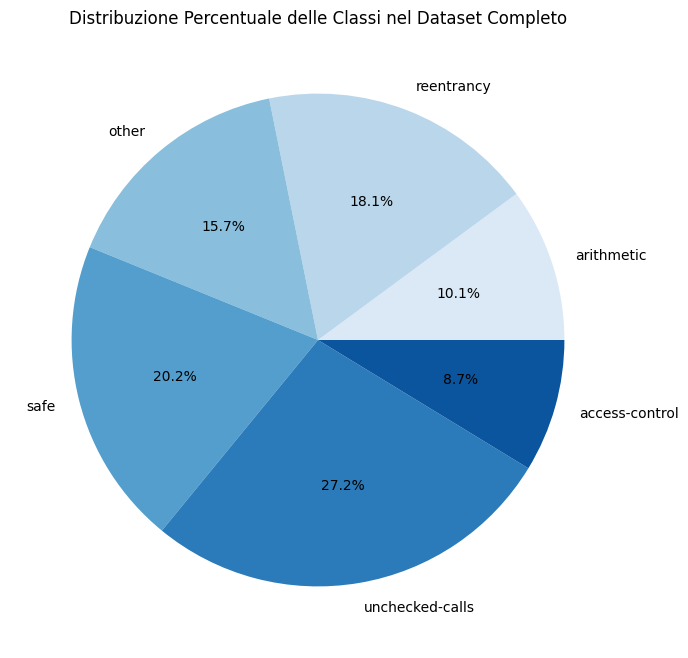
\includegraphics[width=\linewidth]{../../img/class-distribution-relative.png}
      \caption{Distribuzione Percentuale delle Classi}
      \label{fig:relative_distribution}
    \end{subfigure}
    \hspace{0.5cm}
    \begin{subfigure}[b]{0.45\linewidth}
      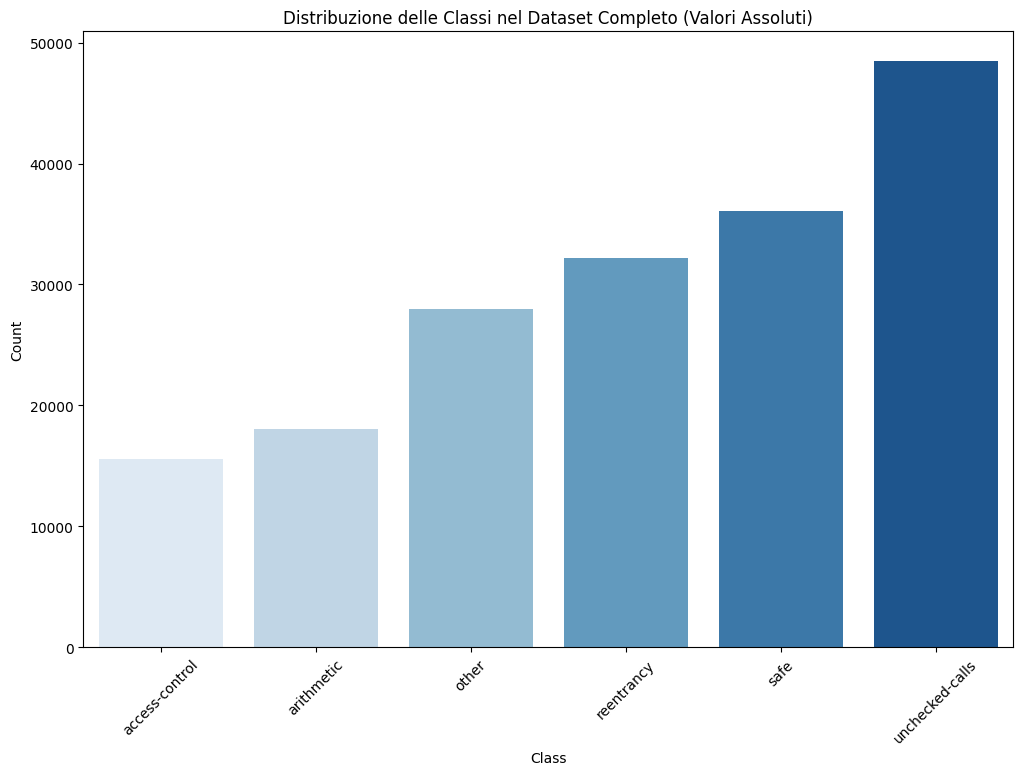
\includegraphics[width=\linewidth]{../../img/class-distribution-absolute.png}
      \caption{Distribuzione Assoluta delle Classi}
      \label{fig:absolute_distribution}
    \end{subfigure}
    \caption{Distribuzioni delle Classi nell'intero dataset, in termini relativi e assoluti.}
    \label{fig:class_distributions}
  \end{figure}

\subsubsection{Matrici di Co-occorrenza}
Le Tabelle \ref{fig:train_cooccurrence_matrix}, \ref{fig:test_cooccurrence_matrix} e \ref{fig:val_cooccurrence_matrix} mostrano le matrici di co-occorrenza per i dataset di addestramento, test e validazione rispettivamente. Le matrici di co-occorrenza indicano la frequenza con cui ogni coppia di classi appare insieme nello stesso elemento.

In questa sezione, vengono presentate le matrici di co-occorrenza per ogni split del dataset, mostrando sia in termini assoluti che relativi il numero di cooccorrenze tra le varie classi.

\begin{figure}[H]
    \centering
    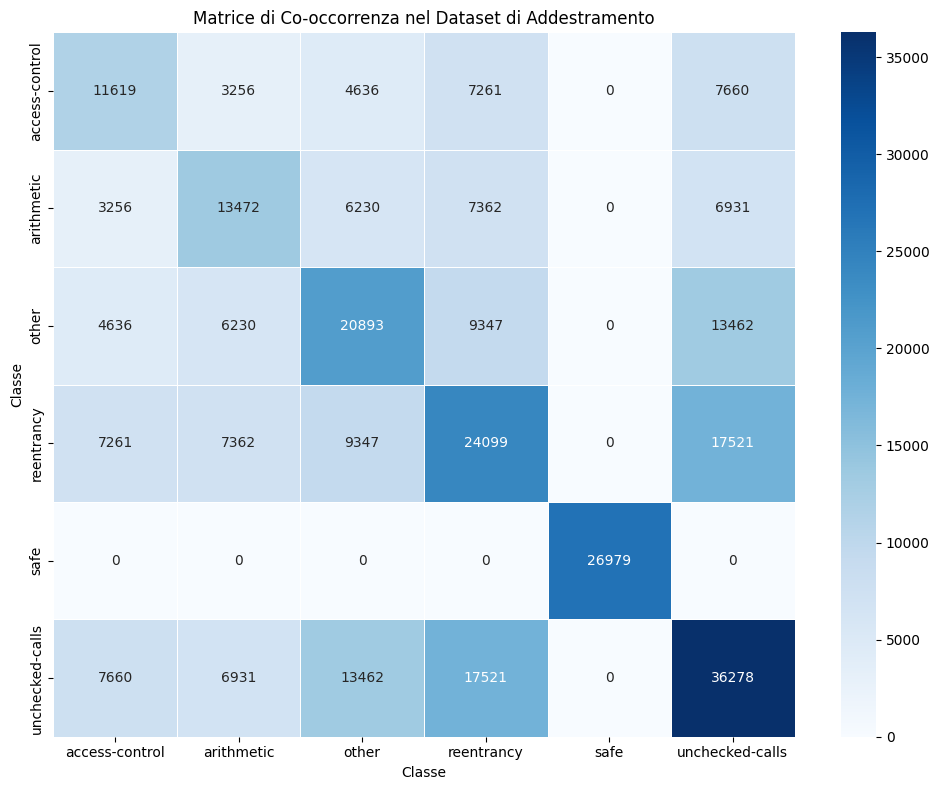
\includegraphics[width=0.7\textwidth]{../../img/TrainCo-occurrency.png}
    \caption{Matrice di Co-occorrenza nel Dataset di Addestramento}
    \label{fig:train_cooccurrence_matrix}
\end{figure}

\begin{figure}[H]
    \centering
    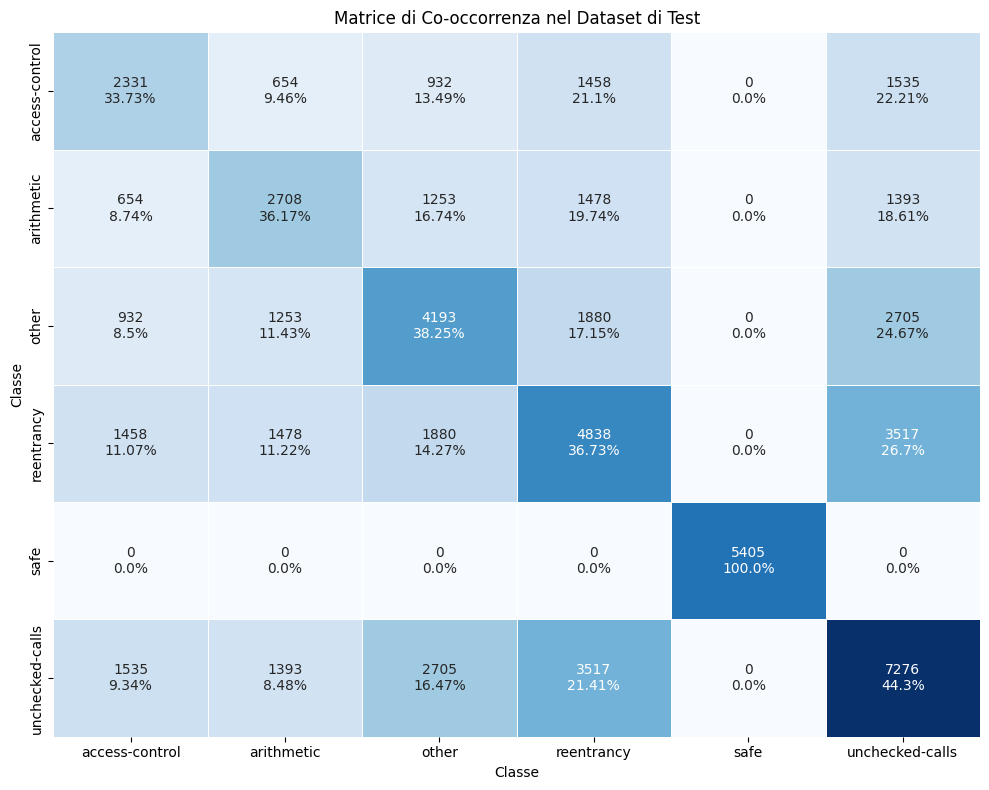
\includegraphics[width=0.7\textwidth]{../../img/TestCo-occurrency.png}
    \caption{Matrice di Co-occorrenza nel Dataset di Test}
    \label{fig:test_cooccurrence_matrix}
\end{figure}

\begin{figure}[h]
    \centering
    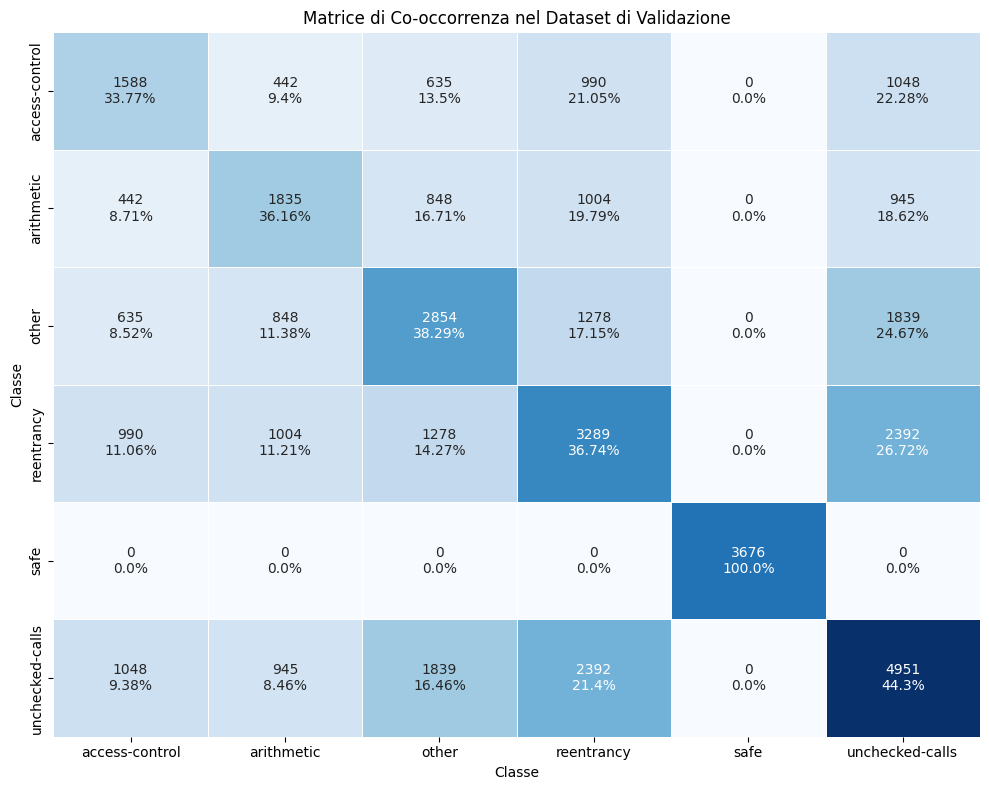
\includegraphics[width=0.7\textwidth]{../../img/ValCo-occurrency.png}
    \caption{Matrice di Co-occorrenza nel Dataset di Validazione}
    \label{fig:val_cooccurrence_matrix}
\end{figure}

Dalla distribuzione delle classi nei diversi dataset, possiamo osservare che:

\begin{itemize}
    \item La classe 'unchecked-calls' è la più frequente in tutti e tre i dataset, con una presenza significativa soprattutto nel dataset di addestramento (36278 occorrenze).
    \item La classe 'access-control' è la meno frequente, con il numero più basso di occorrenze nel dataset di validazione (1588 occorrenze).
    \item Le classi 'safe' e 'reentrancy' sono anche abbastanza rappresentate, specialmente nel dataset di addestramento.
\end{itemize}

Analizzando le matrici di co-occorrenza, notiamo che:

\begin{itemize}
    \item Le classi 'safe' non co-occorrono con altre classi. Questo potrebbe indicare che i dati etichettati come 'safe' sono esclusivamente sicuri e non sovrapposti con altre categorie di vulnerabilità.
    \item Le classi 'unchecked-calls' co-occorrono frequentemente con 'reentrancy', 'other', e 'access-control'. Questo suggerisce che i contratti con chiamate non verificate spesso presentano anche altri tipi di vulnerabilità.
    \item Le classi 'arithmetic' e 'reentrancy' mostrano una co-occorrenza significativa, suggerendo che le vulnerabilità aritmetiche possono spesso essere associate a problemi di rientro.
\end{itemize}

Questi risultati evidenziano l'importanza di considerare la co-occorrenza delle classi quando si analizzano le vulnerabilità nei contratti intelligenti, poiché molte vulnerabilità non si verificano in isolamento ma tendono a manifestarsi insieme ad altre.


\section{BERT}
Il modello BERT (Bidirectional Encoder Representations from Transformers) rappresenta un pilastro fondamentale nel campo del Natural Language Processing (NLP), grazie alla sua capacità di comprensione del contesto delle parole all'interno di una frase o di un testo più ampio. Questo modello, sviluppato da Google, si basa sull'architettura dei transformer, una classe di modelli neurali che ha dimostrato notevole successo nell'analisi del linguaggio naturale.

BERT si distingue per la sua capacità bidirezionale di elaborare il contesto linguistico. A differenza dei modelli NLP precedenti, che processavano il testo in modo sequenziale, interpretando le parole una dopo l'altra, BERT considera sia il contesto precedente sia quello successivo di ciascuna parola all'interno di una frase. Questo approccio bidirezionale consente a BERT di catturare relazioni semantiche più complesse e di fornire una rappresentazione più accurata del significato del testo.

Il funzionamento di BERT può essere compreso attraverso due fasi principali: l'addestramento e l'utilizzo.

Durante la fase di addestramento, BERT viene esposto a enormi quantità di testo, proveniente da varie fonti e domini. Utilizzando un processo noto come "pre-addestramento", il modello apprende i modelli linguistici e il contesto delle parole. Questo pre-addestramento coinvolge due compiti principali: la predizione di parole mascherate e la predizione della successione di frasi. Nel primo compito, BERT impara a prevedere le parole mancanti in una frase fornita, mentre nel secondo compito, il modello apprende a determinare se due frasi sono consecutive in un testo o sono state estratte casualmente da testi diversi.

Una volta completata la fase di addestramento, BERT può essere utilizzato per una vasta gamma di compiti NLP senza la necessità di ulteriori addestramenti specifici. Durante l'utilizzo, il modello riceve in input una sequenza di token, che possono essere parole, frammenti di testo o segmenti di frasi. Ogni token viene rappresentato come un vettore di caratteristiche, derivato dal contesto bidirezionale fornito da BERT durante l'addestramento. Queste rappresentazioni vettoriali possono essere utilizzate per svariati compiti, come classificazione di testo, analisi del sentiment, risposta alle domande, traduzione automatica e molto altro ancora.

In sintesi, il modello BERT ha rivoluzionato il campo del NLP introducendo una comprensione più approfondita e contestualizzata del linguaggio naturale. La sua capacità di catturare il contesto bidirezionale delle parole ha portato a miglioramenti significativi nelle prestazioni dei sistemi NLP su una vasta gamma di compiti e applicazioni. BERT rimane un pilastro fondamentale nell'ambito della comprensione automatica del linguaggio umano, consentendo a macchine e sistemi di interagire e comprendere il linguaggio umano in modo più naturale e preciso.

\end{document}